\documentclass[11pt, compress]{beamer}

\usepackage{preamb}
\usepackage{tikz,tkz-tab}
\usepackage{tkz-euclide}
\usepackage{movie15}
\usepackage{hyperref}
\setbeamertemplate{navigation symbols}{} 
\usetheme{Warsaw}

\setbeamertemplate{theorem begin}{{
\inserttheoremheadfont
\inserttheoremname
\inserttheorempunctuation
}}

\setbeamertemplate{theorem end}{}
\newtheorem{proposition}[theorem]{Proposition}

\theoremstyle{definition}
\newtheorem{mydef}[theorem]{Définition}
\makeatletter

%\captionsetup[figure]{labelformat=empty}
\definecolor{beamer@blendedpurp}{RGB}{241, 148, 138}
 % 0.8,0.2,0.3 rouge carmin presque rose assez élégant avec rgb
 %235 77 77 corail
 % .75 ,.2,.2 rouge clair 
\setbeamercolor{structure}{fg=beamer@blendedpurp}
\setbeamercolor*{palette quaternary}{fg=black,bg=white!80!gray } %bg=couleur à gauche header back
\makeatother
%\setbeamercolor{section in head/foot}{} no touch en fait casse tout
%\setbeamercolor{subsection in head/foot}{fg=black,bg=gray!30} idem 

\makeatletter
\defbeamertemplate*{footline}{shadow theme}
{%
  \leavevmode%
  \hbox{\begin{beamercolorbox}[wd=.5\paperwidth,ht=2.5ex,dp=1.125ex,leftskip=.3cm,rightskip=.3cm plus1fil]{title in head/foot}%
    \usebeamerfont{title in head/foot}\insertshorttitle%
  \end{beamercolorbox}}%
  \begin{beamercolorbox}[wd=.5\paperwidth,ht=2.5ex,dp=1.125ex,leftskip=.3cm plus1fil,rightskip=.3cm]{author in head/foot}%
    \usebeamerfont{author in head/foot}\hfill\insertframenumber\,/\,\inserttotalframenumber
  \end{beamercolorbox}%
  \vskip0pt%
}
\setbeamertemplate{section in toc}{\inserttocsectionnumber.~\inserttocsection}
%\setbeamertemplate{section in toc}{\textcolor{structure.fg}{$\blacktriangleright$}\hspace{1.2 em}~\inserttocsection \\}

%\setbeamertemplate{section in toc}{\inserttocsectionnumber.~\inserttocsection}
\setbeamercolor*{section in toc}{fg=black}
\setbeamercolor*{enumerate item}{fg=black}
\setbeamercolor*{enumerate subitem}{fg=black}
\newcommand*{\rom}[1]{\expandafter\@slowromancap\romannumeral #1@}
\makeatother

%%%%%%%%%%%%%%%%%%%%%%%%%%%%%%%%%%%%%%%%%%%%%%%%%%%%%%%%%%%%%%%%%%%%%%%%%%%%%%%%%
%%%%%%%%%%%%%%%%%%%%%%%%%%%%%%%%%% end styling beamer %%%%%%%%%%%%%%%%%%%%%%%%%%%
\usepackage{tcolorbox}
\newtcolorbox{mybox}{colback=red!5!white,colframe=red!75!black}


\title{Montpellier Network's Package}
\subtitle{Project HMMA$238$}
\author{\vspace*{-1.5cm}Fanchon Herman, Ryma Lakehal et Sahbane Abdesstar}
\date{\vspace*{-2cm}25 Juin 2020}
\institute[Montpellier University]{Montpellier University}
\titlegraphic{%
  \makebox[0.9\paperwidth]{%
    
\includegraphics[scale=.07]{logo_fds.png}%
    \hfill%
    
\includegraphics[scale=.2]{um.png}
    \hspace{.25cm}
  }%
}

\begin{document}

{
\def\mytitleframe{\bgroup
\makeatletter
\setbeamertemplate{footline}
{%
  \leavevmode%
  \hbox{\begin{beamercolorbox}[wd=.5\paperwidth,ht=2.5ex,dp=1.125ex,leftskip=.3cm,rightskip=.3cm plus1fil]{title in head/foot}%
    \usebeamerfont{title in head/foot}\insertshorttitle%
  \end{beamercolorbox}}%
  \begin{beamercolorbox}[wd=.5\paperwidth,ht=2.5ex,dp=1.125ex,leftskip=.3cm plus1fil,rightskip=.3cm]{author in head/foot}%
    \usebeamerfont{author in head/foot}%\hfill\insertframenumber\,/\,\inserttotalframenumber
  \end{beamercolorbox}%
  \vskip0pt%
}
\maketitle
\egroup
\addtocounter{framenumber}{-1}
}
\makeatother
	\mytitleframe
}

\section*{Contents}

\begin{frame}
\frametitle{Table of contents}
  \tableofcontents
\end{frame}

\section[Intro]{Introduction}
\begin{frame}{Introduction}
\begin{block}{}
Package python : \href{https://github.com/fanchonherman/project_network}{\beamergotobutton{Github network}}
\end{block}
\begin{block}{Project subject}
\begin{enumerate}[label=$\bullet$]
    \item videos and widget,
    \item transport: car, bike and walk,
    \item from La Maison du Lez to Place Eugène Bataillon,
    \item shortest path.
\end{enumerate}
\end{block}
\end{frame}

\begin{frame}{Important functions}
\begin{columns}
          \column{0.50\linewidth}
          \begin{enumerate}[label=$\bullet$]
               \item<1-> type\_transport,
               \item<2-> distance\_type\_transport,
               \item<3-> times, 
               \item<4-> animation\_type\_transport.
           \end{enumerate}
           \column{0.50\linewidth}
           \centering
             
\includegraphics[scale=.3]{logo_bike.jpg}
         \end{columns} 
\end{frame}


\section[Visu]{Vizualisation of the shortest path}
\subsection{Walk}

\begin{frame}{Vizualisation of the shortest path}
\begin{block}{}
net.type\_transport('walk')
\end{block}
\begin{figure}[H]
    \centering
    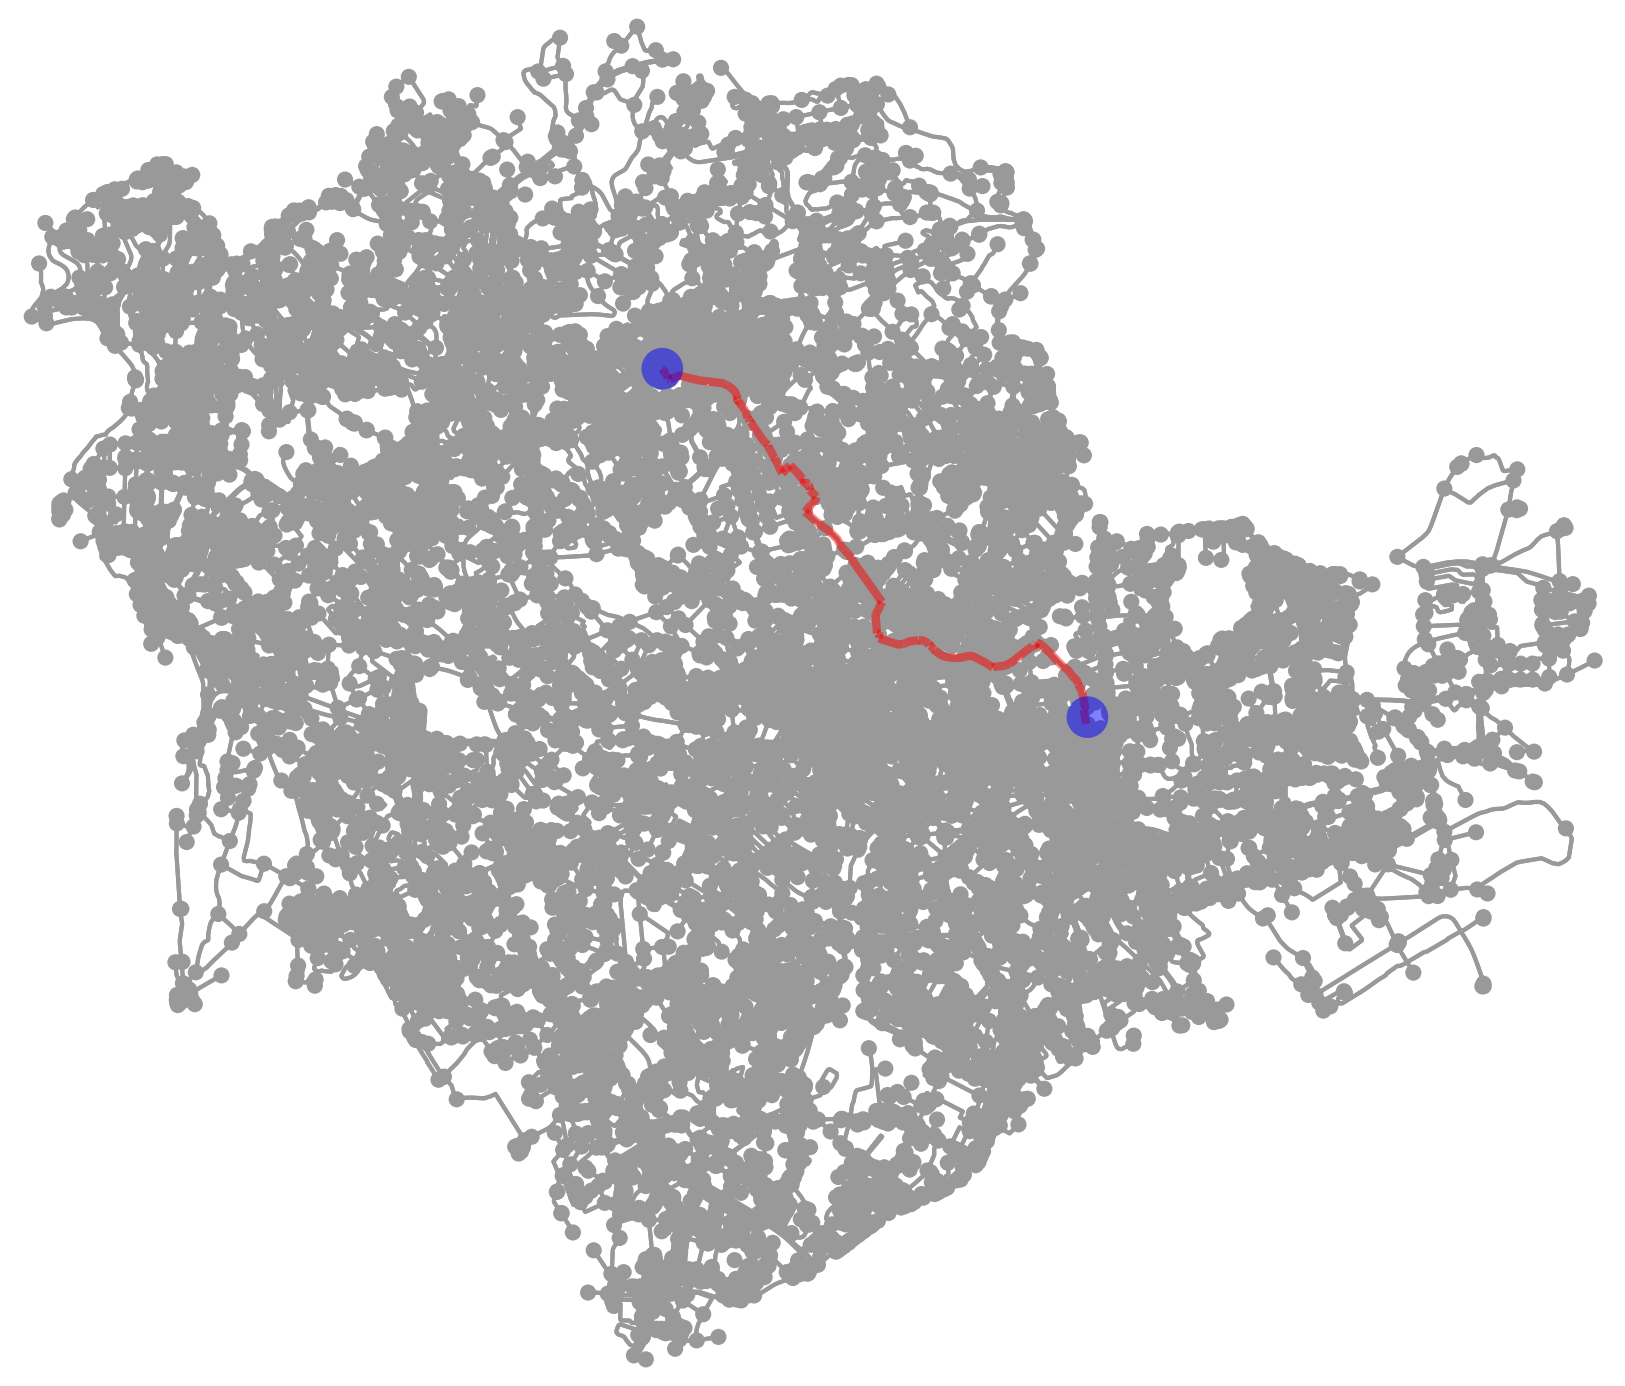
\includegraphics[scale=.45]{walk.png}
    \caption{Vizualisation of the shortest path in walk.}
    \label{fig:walk}
\end{figure}
\end{frame}

\subsection{Car}
\begin{frame}{}
    \begin{block}{}
net.type\_transport('drive')
\end{block}
\begin{figure}[H]
    \centering
    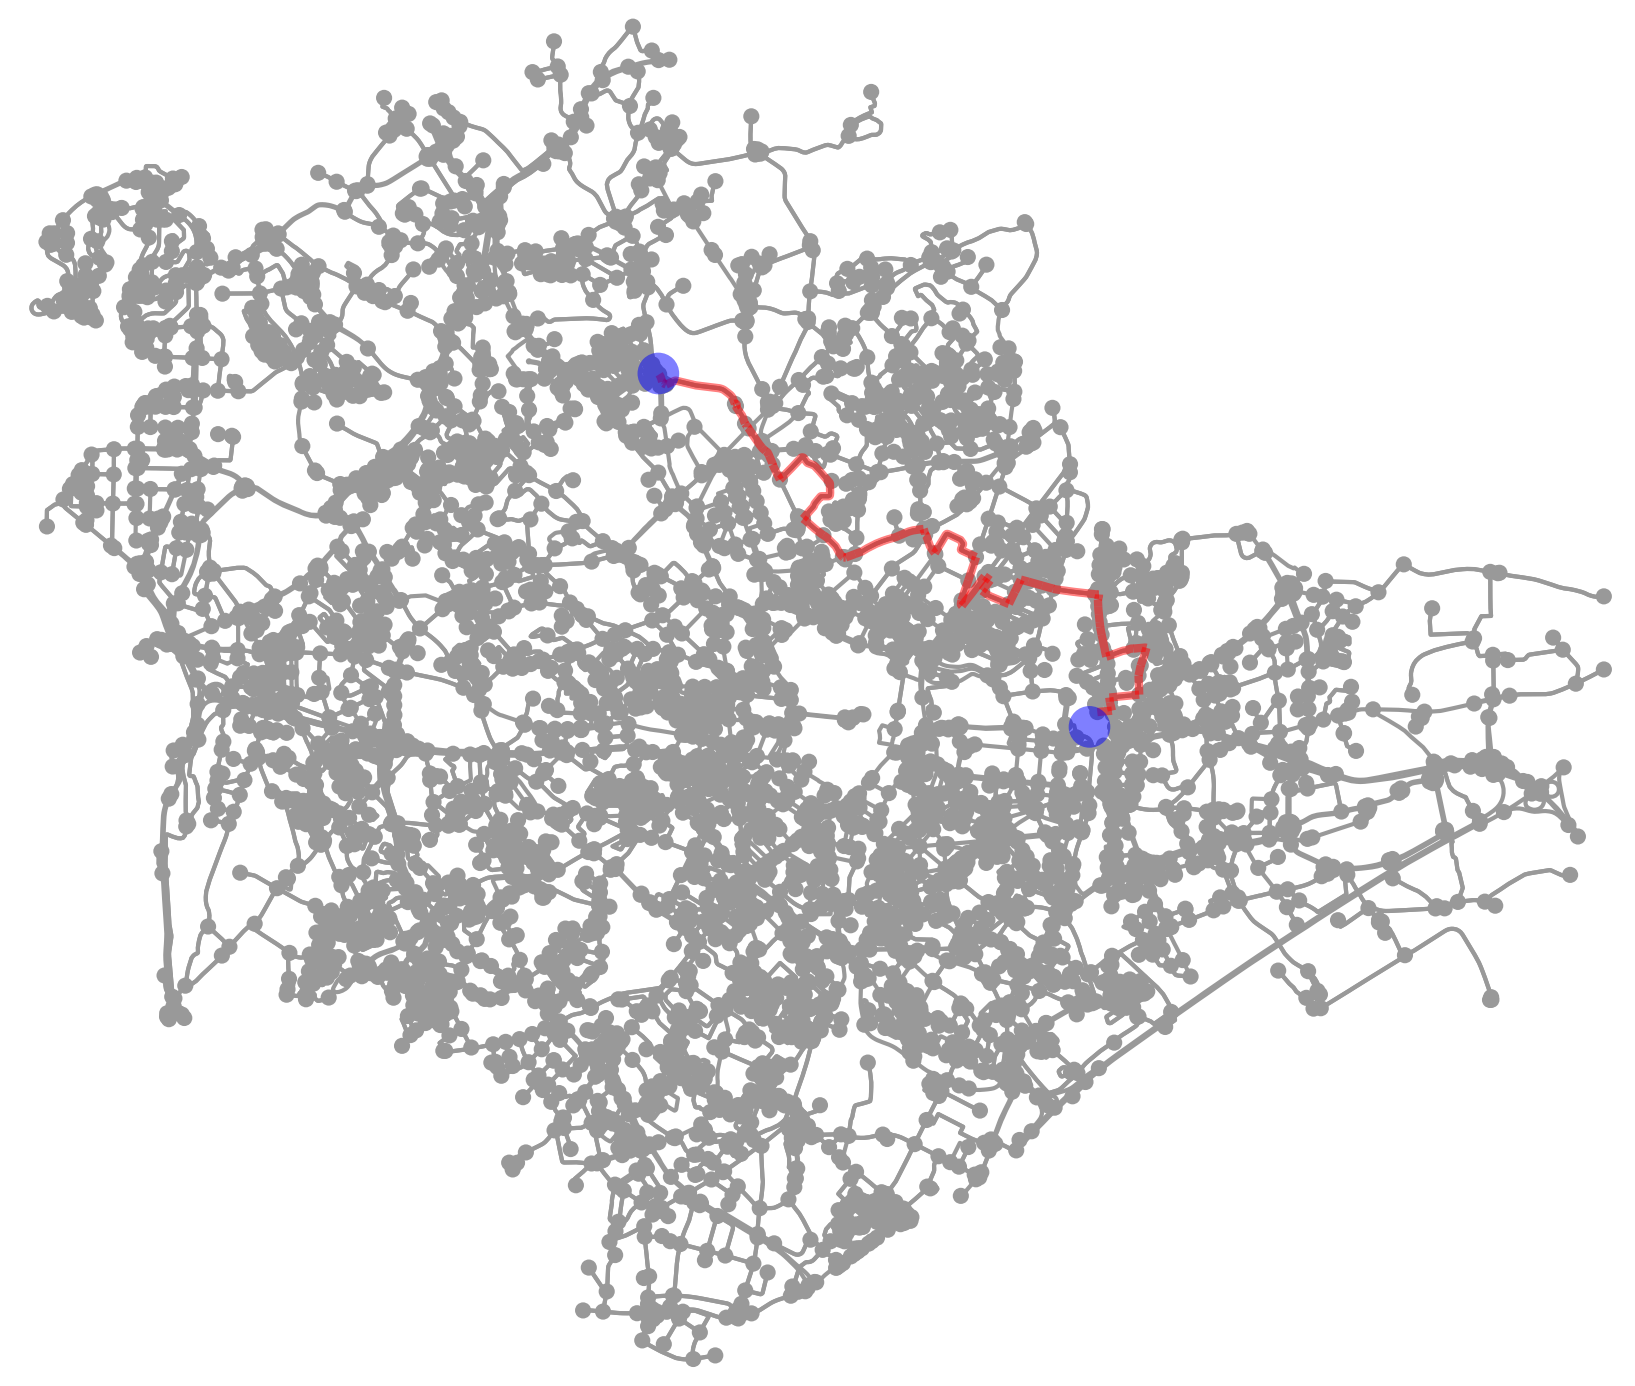
\includegraphics[scale=.45]{drive.png}
    \caption{Vizualisation of the shortest path in car.}
    \label{fig:car}
\end{figure}
\end{frame}

\subsection{Bike}
\begin{frame}{}
\begin{block}{}
net.type\_transport('bike')
\end{block}  
\begin{figure}[H]
    \centering
    
\includegraphics[scale=.4]{bike.png}
    \caption{Vizualisation of the shortest path in bike.}
    \label{fig:bike}
\end{figure}

To see the animations and the widget, click on this link \href{https://github.com/fanchonherman/project_network/tree/master/report}{\beamergotobutton{report}} then launch the notebook.

\end{frame}


\section[Times]{Study time of functions}
\begin{frame}{Study time of functions}
\begin{figure}[H]
    \centering
    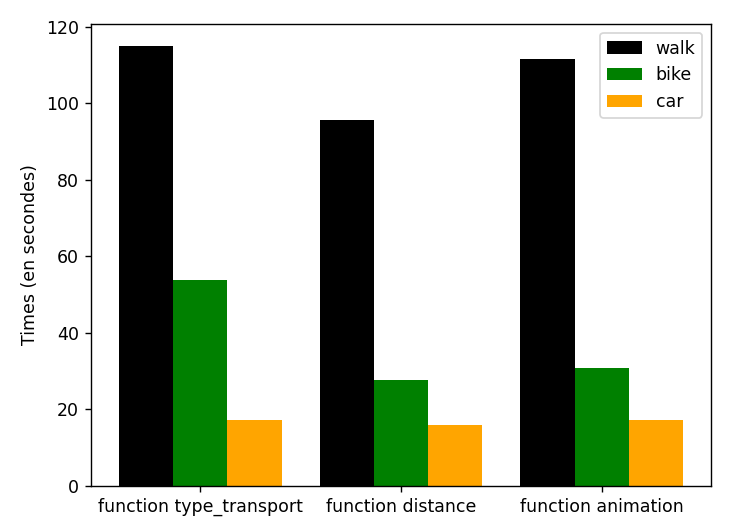
\includegraphics[scale=.5]{histogram.png}
    \caption{Histogram of the time of functions according to the type of transport.}
    \label{fig:histogram}
\end{figure}
\end{frame}

\begin{frame}{Study time of animation function with "TimestampedGeoJson"}
\begin{figure}[H]
    \centering
    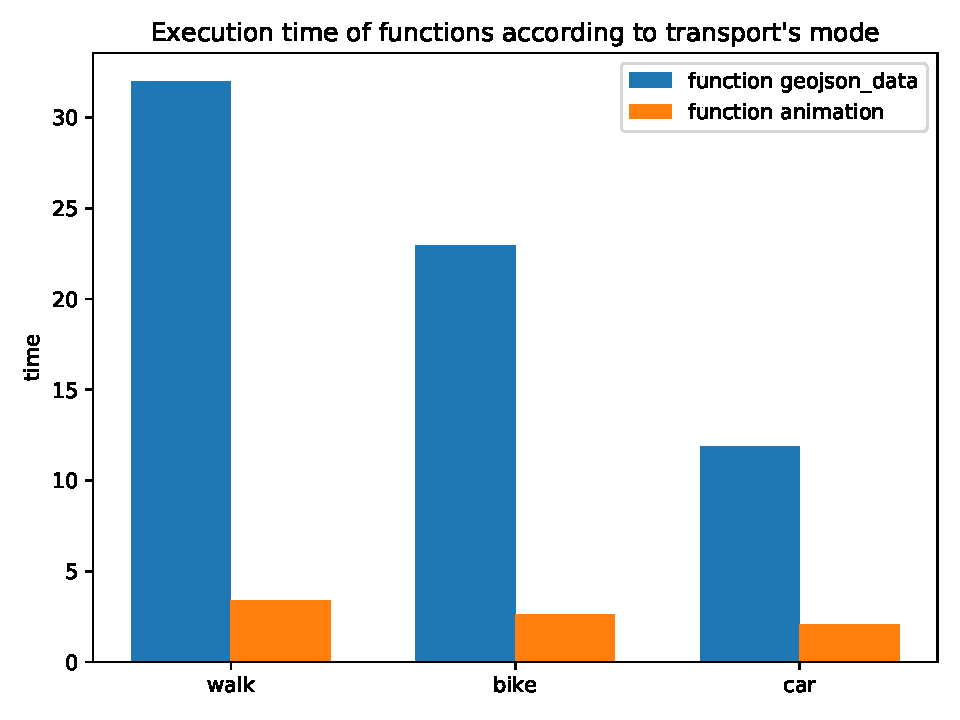
\includegraphics[scale=.5]{GeoJson_histogram.pdf}
    \caption{Histogram of the time of functions according to the type of transport.}
    \label{fig:histogram}
\end{figure}
\end{frame}

\section[Conclu]{Conclusion}
\begin{frame}{Conclusion}
\begin{block}{What we have learnt}
\begin{enumerate}[label=$\bullet$]
    \item osmnx,
    \item networkx,
    \item improvements.
\end{enumerate}
\end{block}

\begin{block}{Upgrades}
\begin{enumerate}[label=$\bullet$]
    \item computation time,
    \item display informations on the map. %ex la vitesse de la personne 
\end{enumerate}
\end{block}
\end{frame}


\end{document}